\section{Before the pandemic}
So we have a picture of most places of worship with little to no online presence, averaging about 65 weekly attendance ~\cite{yonat:shimron} and all of a sudden the whole world is asked to recede to the confines of their homes. Any online presence was mainly used for information dissemination~\cite{helland}. This is because most do not see an online presence as a priority and, in most cases, are limited by the technical know-how of their volunteers. 

An interview with a \textit{masjid} leader of a rural Islamic Center revealed that they only have a \textit{Facebook} page and only use \textit{WhatsApp} for messaging. This rural midwestern town \textit{masjid} was established in 2001 and has been slow to adopt social media. He notes that \textit{WhatsApp} is good for sending out information, but members are often slow to respond. There is a designated social media person in the \textit{masjid}, but the person is a volunteer and has "limited time" to make contributions. The \textit{masjid} has about 50 to 100 people involved with its religious activity counting official members and participating nonmembers. This number is similar to that of its average weekly attendance ~\cite{grant2019religion}. 

\begin{figure}[t!]
\centering
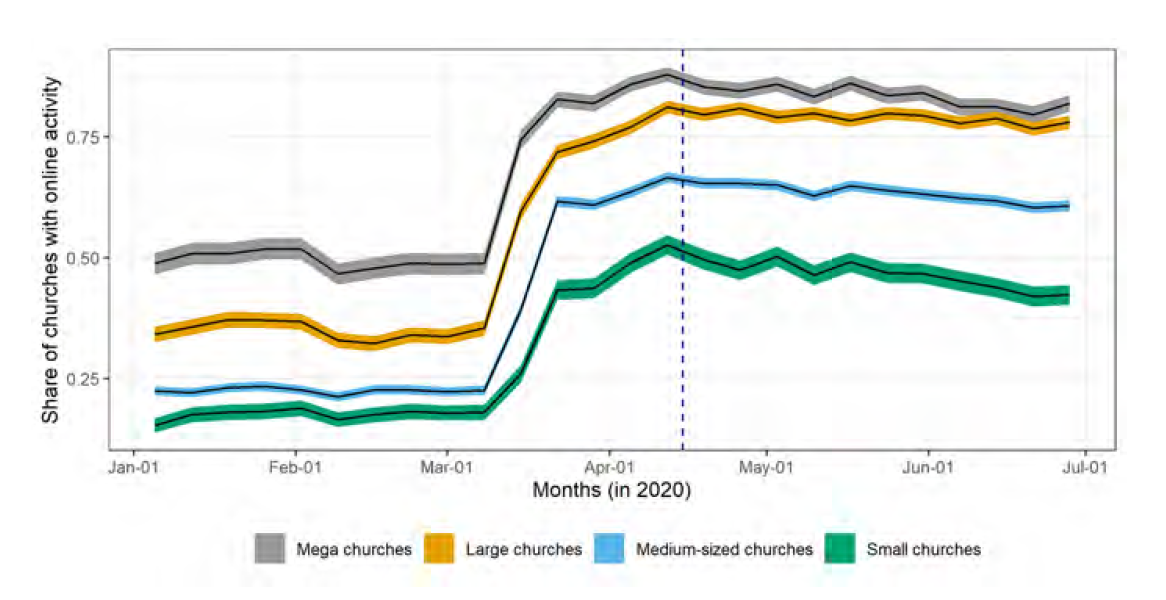
\includegraphics[width=\columnwidth]{images/fig_6.PNG}
\caption{Churches' online activity over time by church size. The dashed line separates the introduction and relaxation periods. Shaded areas indicate the standard deviation, Small churches are defined as receiving up to 50 people on a regular Sunday,
medium churches between 51 and 300, large churches between 301 and 500 and mega churches over 2000.}
\label{fig1}
\end{figure}

\begin{figure}[t!]
\centering
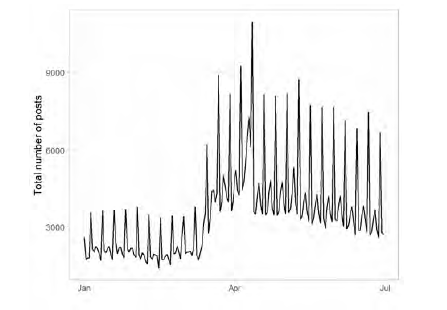
\includegraphics[width=\columnwidth]{images/fig_1.PNG}
\caption{Total number of Facebook posts per day between January 1 and June 30, 2020. Before the pandemic, the maximum number of posts were at 4000. Once the pandemic started, The total number of posts increased significantly.}
\label{fig2}
\end{figure}

\begin{figure}[t!]
\centering
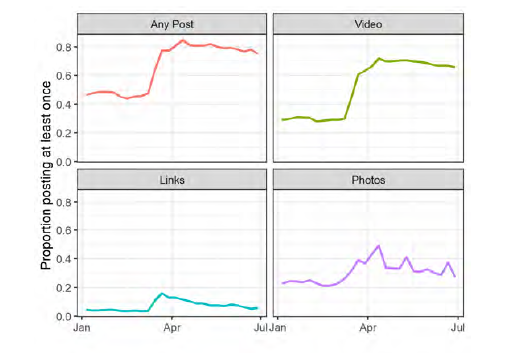
\includegraphics[width=\columnwidth]{images/fig_v3.PNG}
\caption{Proportion of churches that post at least once on Sunday between January 1 and June 30, 2020 overall and by type of post. Video includes live videos (including scheduled and completed live videos), native videos (video files posted directly to Facebook) and YouTube videos. Status describes posts that only contain text.}
\label{fig3}
\end{figure}

\begin{figure}[t!]
\centering
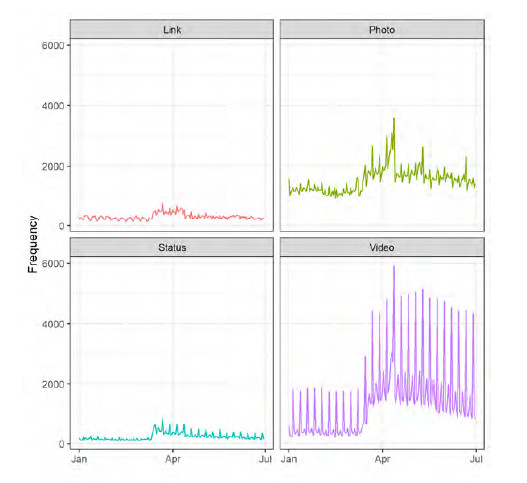
\includegraphics[width=\columnwidth]{images/fig_2.PNG}
\caption{Number of posts made by public U.S. church profiles between January 2020 and June 30 2020 on Facebook by type of post. Video includes live videos (including scheduled and completed live videos), native videos (video files posted directly to Facebook) and YouTube videos. Status describes posts that only contain text.}
\label{fig4}
\end{figure}

The \textit{CrowdTangle Team}, a Facebook-owned tool that tracks interactions on public content from Facebook pages and groups, helped Eva Raiber et. al poll nearly 4000 Christian churches in the United States with a public Facebook profile~\cite{Raiber}. To identify church online activities, they hand-coded 1600 church posts and then used a random forest algorithm to predict the advertisement of online church activity in a Sunday post for the rest of the sample. The prediction algorithm evaluated the type of the post (video, link, live stream, etc), as well as the post text~\cite{Raiber}. As shown in \textbf{Figure~\ref{fig1}}, before the pandemic, the share of the online activities of churches corresponded to the volume of the church. Megachurches averaging over 2000 weekly attendants had more online presence than small churches. As shown in \textbf{Figure~\ref{fig2}}, the total number of posts was, at maximum, 4000. 47\% of churches posted on a given Sunday, as illustrated in \textbf{Figure~\ref{fig3}}. Also, 30\% posted at least one video on a given Sunday before the pandemic and 4\% a link~\cite{Raiber}. The results also show that churches post most on Sunday, the day of worship. In \textbf{Figure~\ref{fig4}}, churches primarily posted videos on Sundays. On weekdays, they are more likely to post a photo~\cite{Raiber}.

Berea Temple International Church, an \textit{Assemblies of God} affiliated church in St. Louis, is no different. Before the lockdown, the church had no official website, no online giving, no live-streamed events, and an under-utilized YouTube channel. Their only active online presence was a Facebook page, which they purely used for information dissemination. Services were held regularly in person every Sunday. Tithes, offerings, and other benevolences were collected in person as well. Sparingly members will mail in their donations by checks. More alarming was the fact that there was no internet connection at the church building. Come May 2020, a citywide mandate was issued requiring everyone to stay home to curb the spread of the virus. Like most places of worship, we had a major problem. How do we keep service going? How do we allow people to keep giving? How do we support our members during this peril? Should we live stream?  

\section{During the heat of the pandemic}
At the onset of the lockdown, the Muslim holy month of Ramadan was just beginning. During the holy month, mosques open their doors each night to members and guests for \textit{iftar} – a communal meal to break the day’s fast~\cite{mulvey}. It’s also one of the most fruitful times of the year for fundraising, particularly for local mosques, which cover the majority of expenses through individual donations. But as in-person worship was put on hold, congregants could no longer share their nightly meal. Throughout the rest of 2020, families were barred from going to Friday prayers, or \textit{Jum’ah}, another robust time for fundraising. Donations to mosques across the country declined dramatically – for some places of worship, annual funding fell by 40-60\%~\cite{mulvey}. To fight this steep decline in funds, many mosques turned to \textit{GoFundMe} to raise funds. The situation got so dire in New York City that Mosaab Sadeia at the Islamic Leadership Council of New York set up a grant for struggling mosques~\cite{mulvey}. 

According to Imam Naeem Baig, outreach director at the Dar Al-Hijrah Islamic Center in Falls Church, Virginia, the mosque live-streamed its Friday nightly prayers. Besides live streaming prayers, the Worcester Islamic Center in Massachusetts also held popular virtual education programs for young people on topics such as what Islam says about the family~\cite{block}.

Millions skipped church during the pandemic. Smaller organizations with older congregations that struggled to adapt during the pandemic were in the greatest danger of a downward spiral from which they couldn't recover. On the Maine coast, the pandemic proved to be the last straw for the 164-year-old Waldoboro United Methodist Church~\cite{sharp}.  Prior to the COVID-19, weekly attendance had dipped to 25 or 30 at the white-clapboard New England church that could hold several hundred worshippers. The number further dwindled to five or six before the final service was held and the church was closed~\cite{sharp}. In Virginia, the Mount Clifton United Methodist Church experienced a similar fate. The church can seat more than 100 but the number of weekly worshippers dwindled to 10 to 15, even before the pandemic. The small white church built on a hill in the Shenandoah Valley in the 1880s may be rented to another congregation, or it may be put up for sale~\cite{sharp}.

In the first few weeks of the pandemic, we turned to Skype to hold our Sunday gatherings online given the 40 minutes limitations with Zoom. To solve the remote giving issue, I built a brand-new website with online giving capabilities. Using Skype for the online gathering was a temporary option as the long goal was to have a functioning live streaming service. However, first, we had to get internet to the main church building. After contracting an electrician, we set up a local network using a custom-built Pfsense router, Cisco switches, and Aruba Access Points across the entire building. This provided the needed internet connection for live streaming. Finally, around November 2020, we live-streamed our first Sunday service on Facebook and YouTube simultaneously; marking a turning point for the history of the local church.

The COVID-19 lockdown in South Africa brought with it particular challenges for the faith communities. All religious gatherings were
banned. Holy Week, Easter, and Pentecost could not be celebrated in the churches~\cite{jerry:pillay}. As expected, this brought huge resistance, since congregating to pray, worship, and celebrate is an integral part of most faiths especially, the Christian faith.

According to \textbf{Figure~\ref{fig3}}, Overall in April, at the height of the pandemic, 82\% of churches posted on a given Sunday, 81\% of Easter Sunday is excluded. 70\% of churches posted at least one video (69\% excluding Easter Sunday) and 11\% a link (10.7\% excluding Easter Sunday). Therefore, nearly twice as many churches posted on a given Sunday in April than did before March 2020. The proportion of churches posting a video more than doubled, as did the number of links~\cite{Raiber}.

\section{Today and onward}
A new Pew Research Center survey finds that Americans are increasingly confident they can safely go to services at a church, temple, mosque or other house of worship. And the percentage who say they actually have attended religious services – in person – in the past month is slightly higher than it was last summer~\cite{smith}. As the pandemic eases, executives say that the hybrid model — in which employees work both remotely and in the office — will become far more common. The majority of executives expect that (for all roles that are not essential to perform on-site) employees will be on-site between 21 and 80 percent of the time, or one to four days per week~\cite{andrea:alexander}. Muslims, who make up about 1\% of the U.S. population, say that they feel blessed that the mosques are open. Imam Naeem Baig, outreach director at the Dar Al-Hijrah Islamic Center in Falls Church, Virginia, was quoted to say, "People are so happy the mosque is open. It gives them an opportunity to see each other and pray together — the feeling of community you can’t get by being at home."~\cite{block}.

The \textit{New York Times} ran a story titled, \textit{"Facebook's Next Target: The Religious Experience"}, early this year highlighting the current landscape of the relationship between religion and social media. Months before the megachurch Hillsong opened its new outpost in Atlanta, its pastor sought advice on how to build a church in a pandemic from Facebook~\cite{colleran}. They wanted to explore what the church would look like on Facebook and what apps they may need: financial giving or live-streaming. Facebook has been cultivating partnerships with a wide range of faith communities over the past few years, from individual congregations to large denominations, like the Assemblies of God and the Church of God in Christ~\cite{colleran}. Facebook's push to be the go-to for religious activities is not surprising. It boasts over 2.8 billion active monthly users, a fertile ground for faith organizations to expand their reach and spiritually influence even more people. However, the sentiment is that virtual religious life is not replacing in-person community anytime soon, and even supporters acknowledge the limits of an exclusively online experience~\cite{colleran}. According to Wilfredo De Jesús, a pastor and the general treasurer for the Assemblies of God, "Online church was never meant to replace the local church. We want everyone to put their face in another book".  This shared sentiment leaves a hybrid approach to religious life in today's world. Most religious organizations, mine included, still maintain pandemic-level online activities like live streaming.

\section{Effects on how we worship}
The COVID-19 pandemic did not initiate the drastic change in how people of different faiths worship. On the contrary, it sped up the change by elevating the urgency to adapt to the new realities.  A survey of 15,278 religious congregations across the United States confirms trends sociologists have documented for several decades: Congregational life across the country is shrinking ~\cite{smith}.  Since I could remember, I have never missed a weekend church service. Born into a protestant family, physically going to church on Sunday was as expected as breathing. As you can imagine, the pandemic brought a drastic change to how personally I had gone about practicing my faith. This sentiment is shared among millions of believers around the world. COVID-19 has inadvertently raised the question of what it means to be the church without going to church. It has called into question our understanding of the church as an institution that is usually associated with buildings, offices, organizational arrangements, budgets, ministry, leaders, theology, doctrine, and visibility~\cite{jerry:pillay}. With the pandemic, churches that kept a connection with congregants and relied less on the physical passing of the plate for donations stood a better chance of emerging unscathed, White-Hammond said~\cite{sharp}.

Michel Lagrée argues that there are two degrees of question in play when addressing the interface between technical change and religion. First-degree effects are those where technology has had a direct impact on religious acts and rituals. That is when the application of technology to the life of the church has produced changes~\cite{260105620200101}. Second-degree effects relate to the prevalent “technical mentality” that seeks to bring the material ease, “which is the very principle behind technical innovation”. Applications towards such ease may bring technology’s central principle into conflict with the church’s “fabric of symbols”, which mark ritualistic religious practice~\cite{260105620200101}.

\subsection{On how we give}
\begin{figure}[t!]
\centering
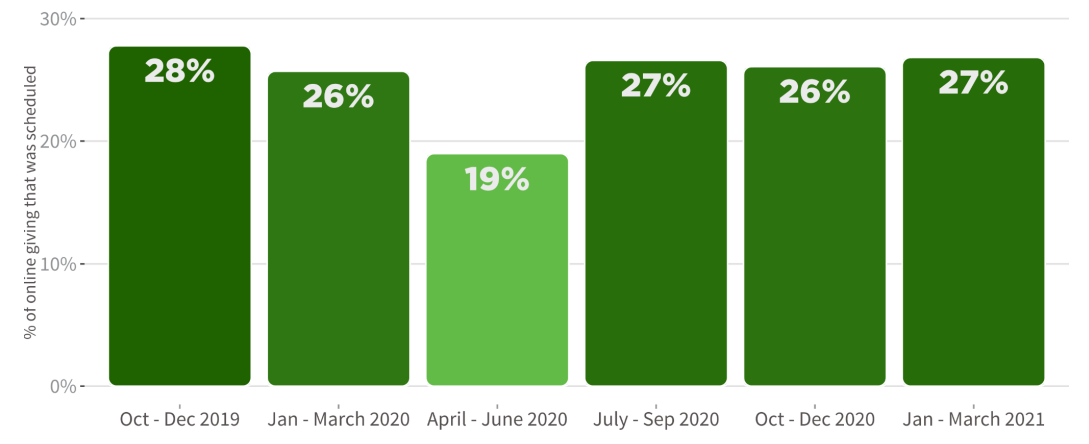
\includegraphics[width=\columnwidth]{images/fig_9.PNG}
\caption{Percentage of online gifts that were scheduled as recurring to churches and ministry organizations in the US during COVID-19}
\label{fig5}
\end{figure}
Places of worship are turning cashless, and we can blame COVID-19 for cementing this change. The measures introduced during the pandemic to limit communal contact forced places of worship to find alternatives for basic rituals like passing the collection box. Now, most faith centers have online options for members to easily send their benevolences using platforms like \textit{Venmo}, text-to-give, and online giving. Tech-savvy members tend to favor this form of donation. All indication shows that this is the way forward for most faith organizations. As congregants have started making their way back to the physical buildings to worship, there has been a shift in their giving behavior. According to a recent report by \textit{Faithlife}, nearly a quarter of 444 surveyed churches reported that they started using online giving for the first time in 2020 ~\cite{jahng}. Of this online giving, 49\% came by mobile giving. As COVID-19 took hold, individual church givers gave more and covered more fees (on average) compared to their pre-pandemic giving~\cite{jahng}. 75\% of all transaction fees were covered by the giver when they had the chance~\cite{jahng}.

Which age group donates the most to charities? A 2018 study found that,  of the 25.9\% of the US population that are Millenials, 26\% gave tribute gifts. 46\% donated to crowdfunding campaigns. 11\% of total US giving comes from Millenials while 84\% of Millennials give to charity, donating an annual average of \$481 across 3.3 organizations. 49\% of all church-giving transactions are made with a card, and 60\% are willing to give to their church digitally. Also, churches that accept tithing online increase overall donations by 32\%. 3 out of 4 people who don’t go to church make donations to non-profit organizations. About 10 million tithers in the US donate \$50 billion yearly to churches and non-profits~\cite{Firch}.

\subsection{On how we pray}
The share of churches that offer an online church activity on a given Sunday more than doubled within two weeks at the beginning of the pandemic (the first half of March 2020) and stayed well above baseline levels~\cite{Raiber}. Prayer is one of the most intimate activities of most religious faiths. The traditional laying of hands in most Christian churches requires the physical presence of both parties (pastor and congregant). Muslims go to the mosque regularly to pray, as do Jews during the sabbath. Today, there is a proliferation of online sites believers can solicit prayers publicly or privately. The visibility of these prayer requests depends on the designs of these websites. However, there is no denying that believers now have another option to virtually request prayers without the need to be physically present. Online forms, social media pages, prayer chat rooms, and live-streamed prayer marathons are some of the mediums available to believers to share their prayer requests.

According to Elizabeth Culliford, the prayer feature is part of Facebook's recent and concerted outreach to the religious community. Facebook sees worshippers as a vital community to drive engagement in its platform. According to Nona Jones, Facebook's head of faith partnerships, the COVID-19 pandemic gave new urgency to this effort after the company saw an increase in people asking each other for prayers during the pandemic. At the end of May, Facebook made its prayer tool, which it had been testing with some faith communities, accessible for all U.S. Facebook Groups to turn on~\cite{Culliford}. According to Fidji Simo, outgoing Facebook app head, one of the biggest communities using Facebook products to connect are people of faith. "When I looked at the data of what was taking off during the pandemic, we were seeing massive growth in the spiritual category.", he said~\cite{Culliford}.

\subsection{On where we fellowship}
In the Philippines, some of the famous religious festivals for the Catholic believers include the devotion to the \textit{Black Nazarene}, the \textit{Sinulog Festival}, or the feast of \textit{Santo Niño de Cebu}, and the re-enactment of the coronation of \textit{Virgen de Los Remedios de Pampanga}. The \textit{Sinulog Festival} attracts millions of attendees who join the penitential walk every year. Thousands of Catholics in Pampanga attend to watch the re-enactment of the coronation of \textit{Virgen de Los Remedios de Pampanga} as well~\cite{gozum}. Religious activities are often reasons why a lot of people gather in one place. However, the pandemic changed that. To observe physical distancing and follow strict lockdowns, religious activities during the COVID-19 pandemic were done virtually. In the Philippines, upon imposition of the quarantine measures, subsequent instructions for local dioceses and parishes were given by the Catholic Bishops’ Conference of the Philippines (CBCP) to hold Masses virtually so that believers could still fulfill their spiritual needs. Even for the Holy Week celebration, believers were asked to stay at home and attend religious activities online so that they would be safe from transmitting the virus~\cite{gozum}. As Corpuz emphasized, “Online platforms as a type of media can be used for the worship of the Church.” These celebrations of online masses and other religious activities were done as a form of adapting to the ‘new normal,’ which is a life with COVID-19~\cite{gozum}. 

Just as in July 2020, eight-in-ten U.S. religious attendees – ranging from 73\% among Catholics to 87\% among those in the evangelical and mainline Protestant traditions – say their congregation is currently recording or streaming its services so that people can watch online or on TV~\cite{smith}. Pastors have for ages encouraged worshippers to ‘come to church and some often resort to making believers feel guilty if they don’t attend church. Needless to say, the closure of churches has turned this around with the plea to ‘please join us on YouTube or other electronic platforms’~\cite{jerry:pillay}. While it is important to recognize the significance of the church ‘gathering to worship’ the pandemic has forced us
to rethink how we gather~\cite{jerry:pillay}.

The COVID-19 lockdown has forced many people to turn to electronic platforms to continue with public worship. This has also provided an opportunity for Christians to be exposed to other forms of worship, liturgical practices, and preaching than they are usually accustomed to. The electronic medium has created opportunities to ‘wander’ and experiment~\cite{jerry:pillay}. For some, it leads to a deeper appreciation of their church tradition and worship practices, and for others, it may have opened up a new world of worship experience altogether~\cite{jerry:pillay}.

\subsection{On the mission of faith institutions}
COVID-19 has opened the eyes of churches to the realities of the sufferings in the world. It has moved churches to orient ministries towards ideals of the kingdom of God rather than the narrow focus on the church. In South Africa, the COVID-19 infections and related deaths are rapidly increasing, over three million people have lost jobs, thousands of businesses have closed or gone bankrupt and millions of people are starving. What is the mission of the church in such a context? It is encouraging to hear inspirational stories of how many churches, against all the challenges of the COVID-19 lockdown rules, are providing food, counseling, prayers, and different ministries to the suffering masses~\cite{jerry:pillay}.

It is pleasing to note that the South African government has come to realize the importance of religious organizations and their role and ability to assist people. The government has designated religious service providers as essential enabling churches to reach out and assist the poor, hungry, needy, and unemployed~\cite{jerry:pillay}. During this time of COVID-19, churches should become centers for solidarity, networks of
compassion, empathy, healing, and emotional support in the face of sickness, fear, pain, and hunger~\cite{jerry:pillay}.

\subsection{On religion as another consumer product}
Merriam Webster dictionary defines \textit{"consumerism"} as the theory that an increasing consumption of goods is economically desirable; a preoccupation with and an inclination toward the buying of consumer goods. So, what does religion has to do with consumerism? In today's age of the internet, where there are prominently two parties involve: one providing a service (provider) and one consuming the service provided (consumer), one can easily see how the increase of the online presence of religious activities easily plays into this established duality of providers and consumers. Now, most religious activities online are free and there is no exchange of goods between parties. However, one cannot ignore that something else is being offered and on the other end is being received. Some have coined the word \textit{"Religious experience"} to refer to this unseen exchange happening everyday on the internet under the religious context. COVID-19 forced every religious organization to offer an online alternative to their members. Now, with faithfuls tuning online to practice their faith to differing degrees, one can clearly see the options it offers to those consuming these religious contents. Reducing the online experience of the members of these religious organizations to a mere exchange of \textit{religious experience} is very simplistic, to some wrong and can be considered a heresy to some. I am quite aware that there is more to it than that and most faithfuls do not tune in to their preferred livestreamed religious service to just get a dose of another religious experience. However, channel flipping has become a new norm for ‘seekers’~\cite{jerry:pillay}. Potter establishes that consumerism has been described as the religion of the 21st century, where everything we do and believe is seen primarily as a consumer choice~\cite{jerry:pillay}. Generally, we would rally against the idea, but Potter reminds us that every churchgoer is a consumer too. We choose where and when we worship, which denomination to follow and the clergy we would like to attend on Sunday. COVID-19 has increased the possibilities of consumer choice and crossed denominational boundaries; worshippers are following preachers they like and are not restricted to church affiliations~\cite{jerry:pillay}.

When everyone is doing the same thing, naturally competition sets in. To stay relevant, one has to be innovative and have a better offering than the guy next door. Most religious organizations are involved a lot in their communities via differing community programs. A lot of these programs are sponsored 90\% of the time via voluntary donations. The internet has shown to be a powerful tool to raise funds for these needed programs. More than ever religious communities are realizing this tool and using it to spread the message of hope, love and urgency. There is no denying that religious organizations play a vital role in the message of "helping the needy". For example, according to Tariq Reqhman, the secretary general of the Islamic Circle of North America, a non-profit in Queens, New York, “99\% of mosques in New York City have community support, and do not have grants or public or government funding. Everything comes from the community.”~\cite{mulvey} According to Mosaab Sadeia at the Islamic Leadership Council of New York, “Ninety-five per cent of small mosques do rely on crowdfunding as their largest source of funding, and they don’t have big financial backers to keep them afloat and keep everything going,”. To him, this is because the Muslim civil society in the US is not developed to the same level as that of the Catholic church, for example, they can only do so much.

\subsection{The ethics of it all}
With most religious institutions live-streaming their services online with music being an important element of it, copyright issues come into play. Religious institutions typically do not need to pay for licenses to play or perform copyrighted music during a worship service; however, this exception does not apply when copyrighted music is recorded or streamed online~\cite{dickson}. Studies have shown that several religious institutions have been subjected to copyright infringement lawsuits for improper streaming and recordings. A clear example of the potential risks and liabilities for copyright infringement occurred in late 2011 when music composer Yesh Music filed a complaint against \textit{First Baptist Church of Smyrna, Tennessee}, seeking a judgment exceeding \$150,000. The church performed two of Yesh’s musical compositions in a worship service live-streamed from its website. More recently, Yesh filed a similar \$3 million lawsuit against renowned \textit{Pastor Joel Osteen and Lakewood Church in Houston, Texas} for streaming Yesh’s song \textit{“Signaling Through the Flames”} during a worship gathering~\cite{dickson}.

Hazik Mohamed, in the article, \textit{Theology, Technology, and Moral Applications: A Muslim Perspective}, discusses how artificial intelligence and other technologies can be developed as a practical moral technology to advance the idea that information technology of morality and ethics is possible~\cite{260105620200101}. Mohamed argues that using artificial intelligence to tackle moral deliberations via creating automated moral systems is inevitable because artificial intelligence systems, by default, are automated problem-solving machines. The tenets of most religious beliefs include the principles of accountability, fairness, justice, and solidarity. However, the lack of fairness in the financial industry led to the disaster of 2008, triggering the creation of Bitcoin. The authors of Bitcoin noted that “their design sacrificed efficiency to ensure that theft would not pay because rewriting the Bitcoin ledger would require so much computational power”~\cite{260105620200101}. Thanks to blockchain, two people who do not know each other can make a transaction with a high level of trust. The decentralized nature of this technology makes it impossible for an entity to control it for its ill gains.

The saying "One should treat others as one would like others to treat oneself" is regarded as the \textit{Golden Rule}. Walter Terence Stace argued that the Golden Rule was much more than simply an ethical code. It is in some form in almost every ethical tradition including, the Three Laws of Robotics, UNWC convention, All belief systems, and Technical Codes and Conventions. While it is relatively straightforward to define ethics and morality, it is less obvious when actions are faced with complex dilemmas~\cite{260105620200101}. The classical Trolley Problem is one such complex hypothetical dilemma. The problem presents five people on board a trolley screaming for assistance: the trolley’s brakes have failed, and the vehicle is seemingly out of control and unable to stop. However, there is a hand lever to switch the tracks. The hand lever can veer the trolley into a sandpit, potentially providing safety for the trolley’s five passengers. But there is a problem: along this track leading to the sandpit stands a man unaware of the trolley’s problem. There is no time or means to warn him to get out of the way. The passengers may be saved by pulling the lever and guiding the trolley to safety, but the man could die. The trolley problem raises an ethical dilemma to consider how an action, and that the consequences of that action, have moral implications. But exactly which consequences are allowable?~\cite{260105620200101}

According to Aquinas, an evil act is never justified by a greater good, even though five people’s lives would be saved as a consequence. Aquinas also used a form of self-defense argument to support his position here. That is, as long as the victim’s intent is to save his or her own life (a good intent), and not to kill his or her attacker (an evil intent), then the act of self-defense is justifiable. Immanuel Kant believed that morality is connected to reason and that the rightness or wrongness of actions does not depend on their consequences, but on whether they fulfill our duty. Hence, if we applied Kant’s views to pulling the lever to divert the trolley, which then incidentally kills an innocent man, it is allowable if it saves five people~\cite{260105620200101}.

Mohamed goes on to say that if morality is reason-based, then it can be codified for machines to act in ways that we see as morally right. But if it is instinctive or highly influenced by circumstantial emotions, such elements will be difficult to be captured and assimilated into technology. Such a remapping of intellectual and imaginative possibilities for the integration of scientific functionality may be extremely challenging~\cite{260105620200101}.

